
\section{Methodology}
To measure the SIDIS cross section presented above, one needs a source of high energy electrons, a detector system capable of measuring the final state electron and hadron, and a computing cluster to perform data processing and analysis.  All of these facilities are provided by Jefferson National Lab, which houses an electron accelerator known as CEBAF, the CLAS spectrometer for detection, and a moderate sized computing cluster for data processing.  In addition to these facilities, a set of analysis techniques and procedures is needed to complete this thesis study.  This section details the methodology used to complete this thesis, comprised of the experimental facility and procedure as well as the data analysis procedure.

\subsection{Experimental Facility}
Jefferson Lab is home to the Continuous Electron Beam Accelerator Facility (CEBAF).  It houses 4 state of the art experimental end-stations for fixed target collisions of electrons or photons on various targets.  CEBAF begins with a 45-MeV electron injector.  The accelerator consists of two linear accelerators (north and south LINACs) and a pair of recirculating arcs at either end of the race track shaped facility.  CEBAF was designed to generate up to 6 GeV electron beams, and has now been upgraded to provide 12 GeV electrons. 

\subsubsection{CLAS in Hall-B}
Hall-B contains the CEBAF Large Acceptance Spectrometer (CLAS) a large spherical detector capable of measuring final state particles with a large range of momentum and angles.  CLAS has the ability to measure exclusive reactions, reconstructing the 4-vectors of all final state particles involved in the reaction.  In cases where one particle is not detected, CLAS also has the resolution to resolve them from missing mass spectra.  This is achieved by combining several different types of detectors into one package, which will be described below.  The CLAS detector has now been dismantled and replaced with CLAS12, but the following sections describe CLAS as it was at the time of data taking for the E1-F experiment used in this thesis.\\

The major components of CLAS \cite{clas} are designed to identify different types of particles at different ranges of momenta, they are:

\begin{figure}
  \centering
  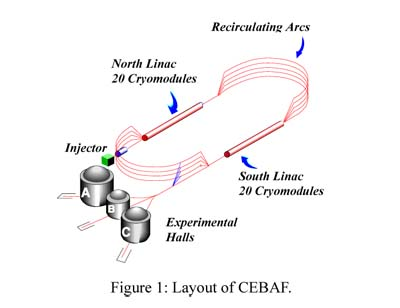
\includegraphics[width=6cm]{image/cebaf.jpg}
  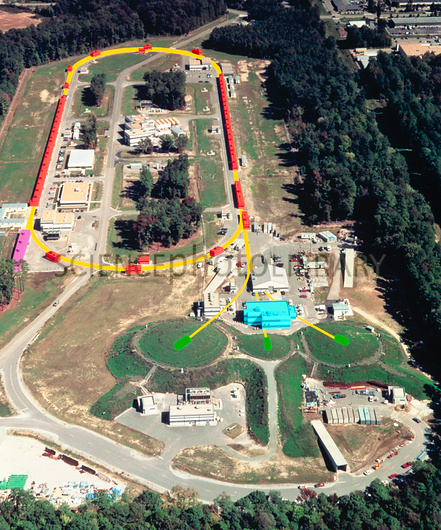
\includegraphics[width=4cm]{image/jlab-photo.jpg}
  \caption{ Left: Diagram showing how CEBAF is constructed.  Right: Jefferson Lab shown from above with the accelerator labeled as well as the experimental end stations.}
  \label{fig:jlab}
\end{figure}

\begin{itemize}
\item Large Torus Magnet - The torus is the central bending magnet which creates a toroidal magnetic field and dictates the design of almost all other detectors.  The torus consists of 6 superconducting coils, (operated at up to 3860 Amperes) which seperate the forward detector systems into 6 distict sectors.  The torus magnet can be used to bend charged particles toward or away from the beamline, and creates the field necessary to determine charge and momentum of particles incident on the CLAS detectors.  
\item Drift Chamber systems - A total of 18 drift chambers are used, 3 radially seperated chambers per sector which are refered to as ``Regions 1-3''.  The primary role of the drift chambers is to provide charge identification and momentum by measuring the bend of the particle as it passes through the known magnetic field.    
\item Cherenkov Light Counters - CLAS is equipped with 6 Cherenkov light counters, filled with $C_{4} F_{10}$.  The Cherenkov Counters (CC) serve two purposes.  The CC serves as a trigger for electrons, and also separates electrons from negative pi-mesons $\pi^{-}$ below 2.5 GeV/c.
\item Scintillating Time Of Flight Panels - Scintillating time of flight (TOF) counters offer coverage from $8^{\circ} - 142^{\circ}$ in the polar angle.  The primary function of the TOF system is to provide timing information to differentiate between particles of different mass based on their time of flight and momentum.  
\item Electromagnetic Calorimeter - The last layer of detection is the electromagnetic calorimeter (EC), which consists of alternating layers of lead and scintilation material.  Electrons and photons can be detected from the shower they leave behind as they pass through the EC.  The EC was designed to have a layered structure, so as to provide hit position information as the particle passes through each layer.  The EC is vital in reconstructing neutrals which strongly decay into photons (such as $\pi^0, \eta$). See figure \ref{fig:ec_clas}.  
\end{itemize}

\begin{figure}
  \centering
  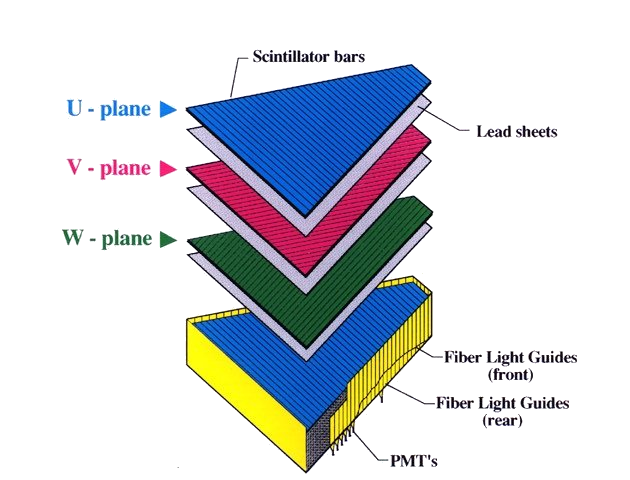
\includegraphics[width=5cm]{image/ec.png}
  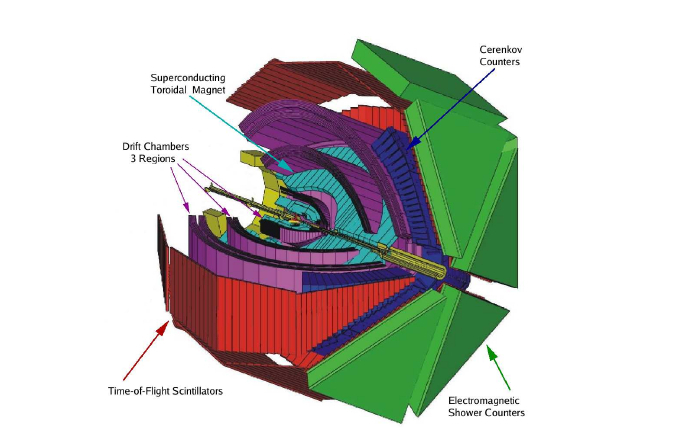
\includegraphics[width=5cm]{image/clas.png}
  \caption{ Left: The CLAS electromagnetic calorimeter, Right: Computer Rendering of CLAS with detector subsystems labeled.}
  \label{fig:ec_clas}
\end{figure}

\subsection{Data Analysis}
The process of taking raw data from the experiment and producing accurate cross sections is a technically challenging and software intensive process.  Only the most salient and physically motivated details will be described here as to give the reader an accurate picture of the procedures employed in this dissertation.  \\ 

Data analyses consist of several important steps:

\begin{itemize}
\item Data Preparations (reconstruction, corrections)
\item Particle Identification
\item Event Selection
\item Acceptance Corrections
\item Radiative Corrections
\end{itemize}

\begin{figure}
  \centering
  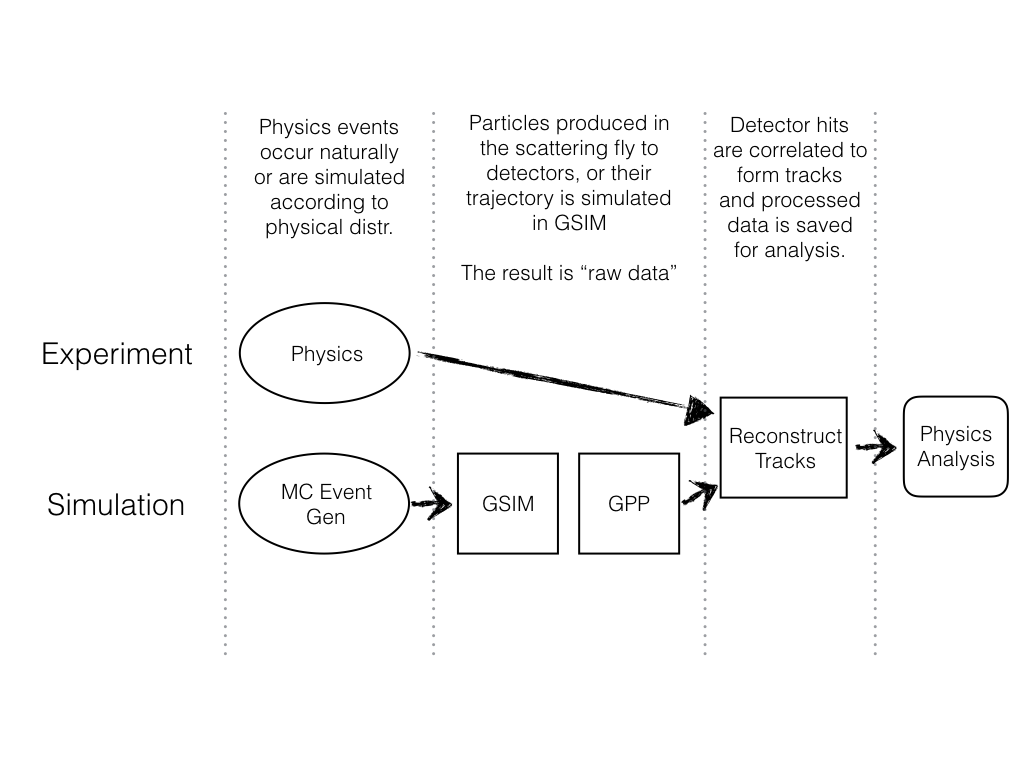
\includegraphics[width=10cm]{image/dataflowchart.png}
  \caption{Comparison of the life of experimental data and monte carlo simulated data.}
  \label{fig:dataflow}
\end{figure}

\subsubsection{Reconstruction of Raw Data}
The result of an experiment is simply a collection of ``snapshots'' or readings from the large array of electrical sensors which comprise CLAS.  These electrical signals have to  be interpreted as particles, and this complicated task is done with reconstruction software called RECSIS.  Accurate maps of the toroidal magnetic field in the hall are used in conjuction with the detector hits to reconstruct particle tracks through CLAS.  \\

\subsubsection{Particle Identification \& Event Selection}
The reconstruction (RECSIS) software applies preliminary and rough particle identication methods to the data, most analyses then apply a more sophisticated particle analysis package to have more control over the final event sample.  All experiments identify electrons in order to calculate kinematic quantities for each reaction, and for this analysis we further identify photons (which are we later attribute to decayed $\pi^{0}$ mesons).  The dominant decay mode for $\pi^0$ mesons is $\pi^{0} \rightarrow \gamma \gamma$ with a branching ratio of approximately 99\%. \\

Particle Identification techniques almost always rely on placing cuts on values of detector responses for each hit.  The cuts used to identify electrons are summarized below.

\begin{itemize}
\item $q < 0$ Determined from the direction of bend in the magnetic field, eliminates neutral and positive particles.
\item $\frac{E_{dep}}{p}$ in the EC, which probes $\frac{dE}{dx}$ and for certain ranges of momenta can eliminate heavier negative particles ($\pi^-$).
\item $CC$ signal is present, which removes low momenta heavier negatives.
\end{itemize}

In addition to particle specific cuts, all particles are subject to geometric cuts which remove hits close to detector edges or remove hits from shadows of other detectors.  Hits near the edges of the electromagnetic calorimeter can partially shower outside of the detector, and the energy is incorrectly reconstructed.  

\begin{figure}
  \centering
  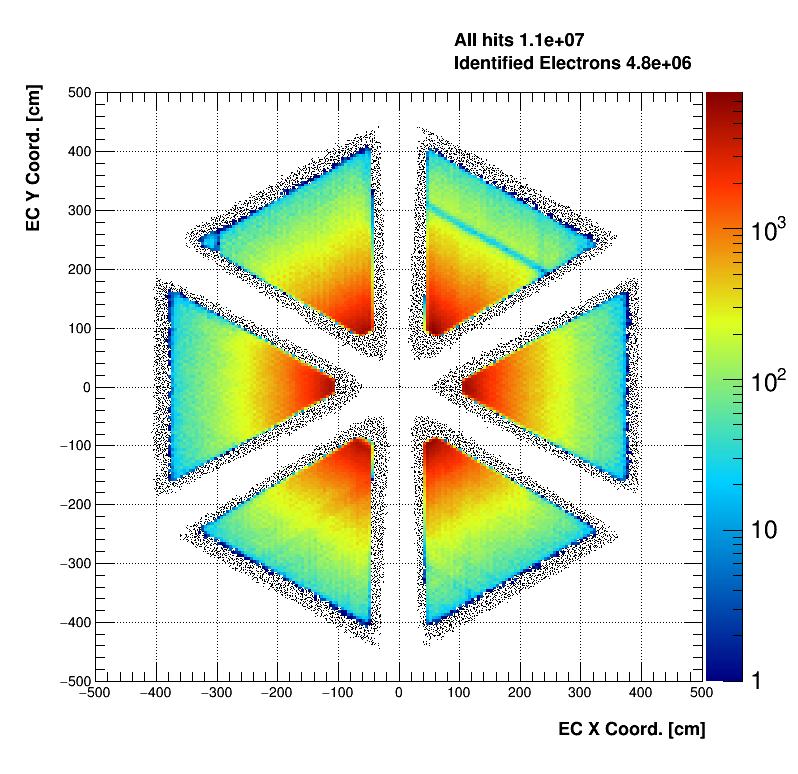
\includegraphics[width=8cm]{image/ECFiducial.png}
  \caption{Electromagnetic (EC) calorimeter negative track hits.  Shown in black, negatives tracks rejected in electron identification.  Hits close to the borders of the EC imcompletely shower and can reconstruct with incorrect energy.}
  \label{fig:ecfid}
\end{figure}

After particle identification, kinematic cuts are used to select the physics of interest from the variety of processes that produce the same set of final state particles.  As an example, one might imagine performing electron identification and then using a cut on the invariant mass of the final state $W$ to separate elastic events (in which $W = M_{proton}$) from higher W inelastic scattering events.  For selection of SIDIS events we use several kinematic cuts.

\begin{itemize}
\item{$W > 2.0 \, GeV/c^{2}$ - This cut ensures that the measurement is performed in the DIS region.}
\item{$Q^{2} > 1.0 \, GeV^{2}/c^{2}$ - A typical cut on $Q^{2}$ which tries to ensure the analysis is done in the region where perturbative QCD and factorization applies.}
\item{$y < 0.7$ - A cut on y is used to suppress the contribution from radiative effects.}
\end{itemize}

\subsubsection{Acceptance Corrections}
Monte Carlo methods are incorperated into almost every analysis in particle physics, and are often used to predict results of coming/proposed experiments.  In this analysis, monte carlo events that follow physical distributions are generated to calculate detector acceptance and do radiative corrections.\\

Due to physical restrictions of the detector (edges, obstructions, and holes) as well as inefficiencies, the number of events reconstructed is not in general the true number of events which occured in the experiment.  Moreover, while holes and obstructions may be quite obvious in angular or spatial distribtutions, thier effects on kinematic distributions is highly non-trivial.  In order to correct for this effect, the detector acceptance is calculated.  First, a large sample of events are generated and the true kinematics are saved.  These events are swam through the detector in a simulation known as GSIM (based on the CERN GEometry ANd Tracking package version 3).  The output of GSIM is then comparable to the raw data from the experiment.  One additional step is performed before reconstruction that smears the resolution in the drift chambers and time of flight to match experimentally measured parameters.  The simulated data is then reconstructed in the same way as data using recsis.  Acceptance is defined as the ratio of reconstructed events in each bin to the number of generated events in that bin.

\begin{equation}
  A_{i} = \left( \frac{N_{rec}}{N_{gen}} \right)_{i}
\end{equation}

\begin{figure}
  \centering
  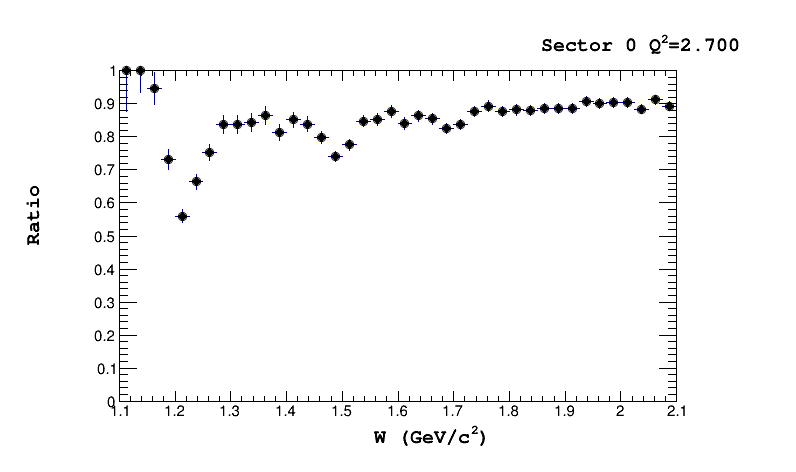
\includegraphics[width=5cm]{image/acceptanceSector0Slice4.png}
  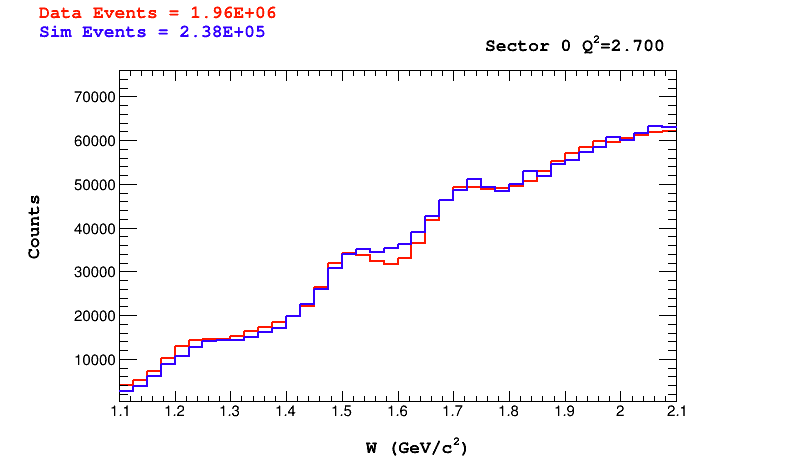
\includegraphics[width=5cm]{image/compareDataSimSector0Slice4.png}
  \caption{Left: Acceptance for one $Q^{2}$ bin shown as a function of W.  Right: Comparison between data and reconstructed events. }
  \label{fig:acceptance}
\end{figure}

Here the subscript $i$ reminds the reader that the acceptance ratio is calculated in each bin.  

\subsubsection{Radiative Corrections}

Radiative effects such as initial or final state radiation alter the kinematics of events and lead to shifts in kinematic quantities.  It is standard practice to calculate and publish Born cross sections (without radiative effects).  Typically, a set of monte carlo generators (with/without radiative effects) is used to create a correction factor for each bin to correct for radiative effects.  We define the correction factor:

\begin{equation}
  R_{i} = \left( \frac{N_{Gen}^{rad}}{N_{Gen}^{norad}} \right)_{i}
\end{equation}

